\documentclass[letterpaper, 12pt]{article}

\usepackage{tabularx}
\usepackage{amsmath}  
\usepackage{physics}
\usepackage{graphicx} 
\usepackage[portuguese]{babel}
\usepackage[margin=1in,letterpaper]{geometry} 
\usepackage{cite} 
\usepackage[final]{hyperref} 
\hypersetup{
	colorlinks=true,       
	linkcolor=blue,        
	citecolor=blue,        
	filecolor=magenta,     
	urlcolor=blue         
}

\begin{document}

\title{\bf Amplificadores}
\author{Gabriel Wendell Celestino Rocha\footnote{\href{mailto:gabrielwendell@fisica.ufrn.br}{gabrielwendell@fisica.ufrn.br}}}
\date{\today}
\maketitle

\begin{abstract}
Resumo do experimento abordado neste relatório. Deve conter uma descrição bastante breve e geral dos \textbf{objetivos} do experimento, os \textbf{métodos} utilizados para a coleta dos dados e posterior tratamento dos mesmos, os \textbf{resultados} obtidos e a \textbf{conclusão} do relatório.
\end{abstract}



%%%%%%%%%%%%%%%%%%%%%%%%%%%%%%%%%%%%%%%%%%%%%%%%%%%%%%
\section{Introdução}\label{Sec 1 - Introdução}
Uma importante aplicação dos transistores é a de amplificação de um sinal AC. Para amplificar um sinal AC devemos garantir a operação DC do transistor na região linear ativa. O circuito que assegura está condição é chamado de \textbf{Circuito Universal de Polarização} (CUP). Tal tipo de circuito é usado para manter as condições de operações constantes.

O amplificador emissor comum é um dos blocos mais utilizados em projetos integrados, apresentando características de ganho de corrente, ganho de tensão, impedância de entrada e impedância de saída bastante flexíveis e úteis.



%%%%%%%%%%%%%%%%%%%%%%%%%%%%%%%%%%%%%%%%%%%%%%%%%%%%%%
\section{Embasamento teórico}\label{Sec 2 - Teoria}
O modelo de pequenos sinais ($ac$) deste tipo de amplificador é apresentado abaixo onde:
\begin{equation}
    g_{m}=\frac{I_{C}}{V_{T}};
\end{equation}
\begin{equation}
    r_{\pi}=\frac{\beta}{g_{m}};
\end{equation}
\begin{equation}
    r_{0}=\frac{V_{A}}{I_{C}}.
\end{equation}

No modelo de grandes sinais vemos que, para $V_{i}$ variando de 500 mV até cerca de 800 mV, o transistor $Q_{1}$ vai do corte até a saturação.

\begin{figure}[h]
    \centering
    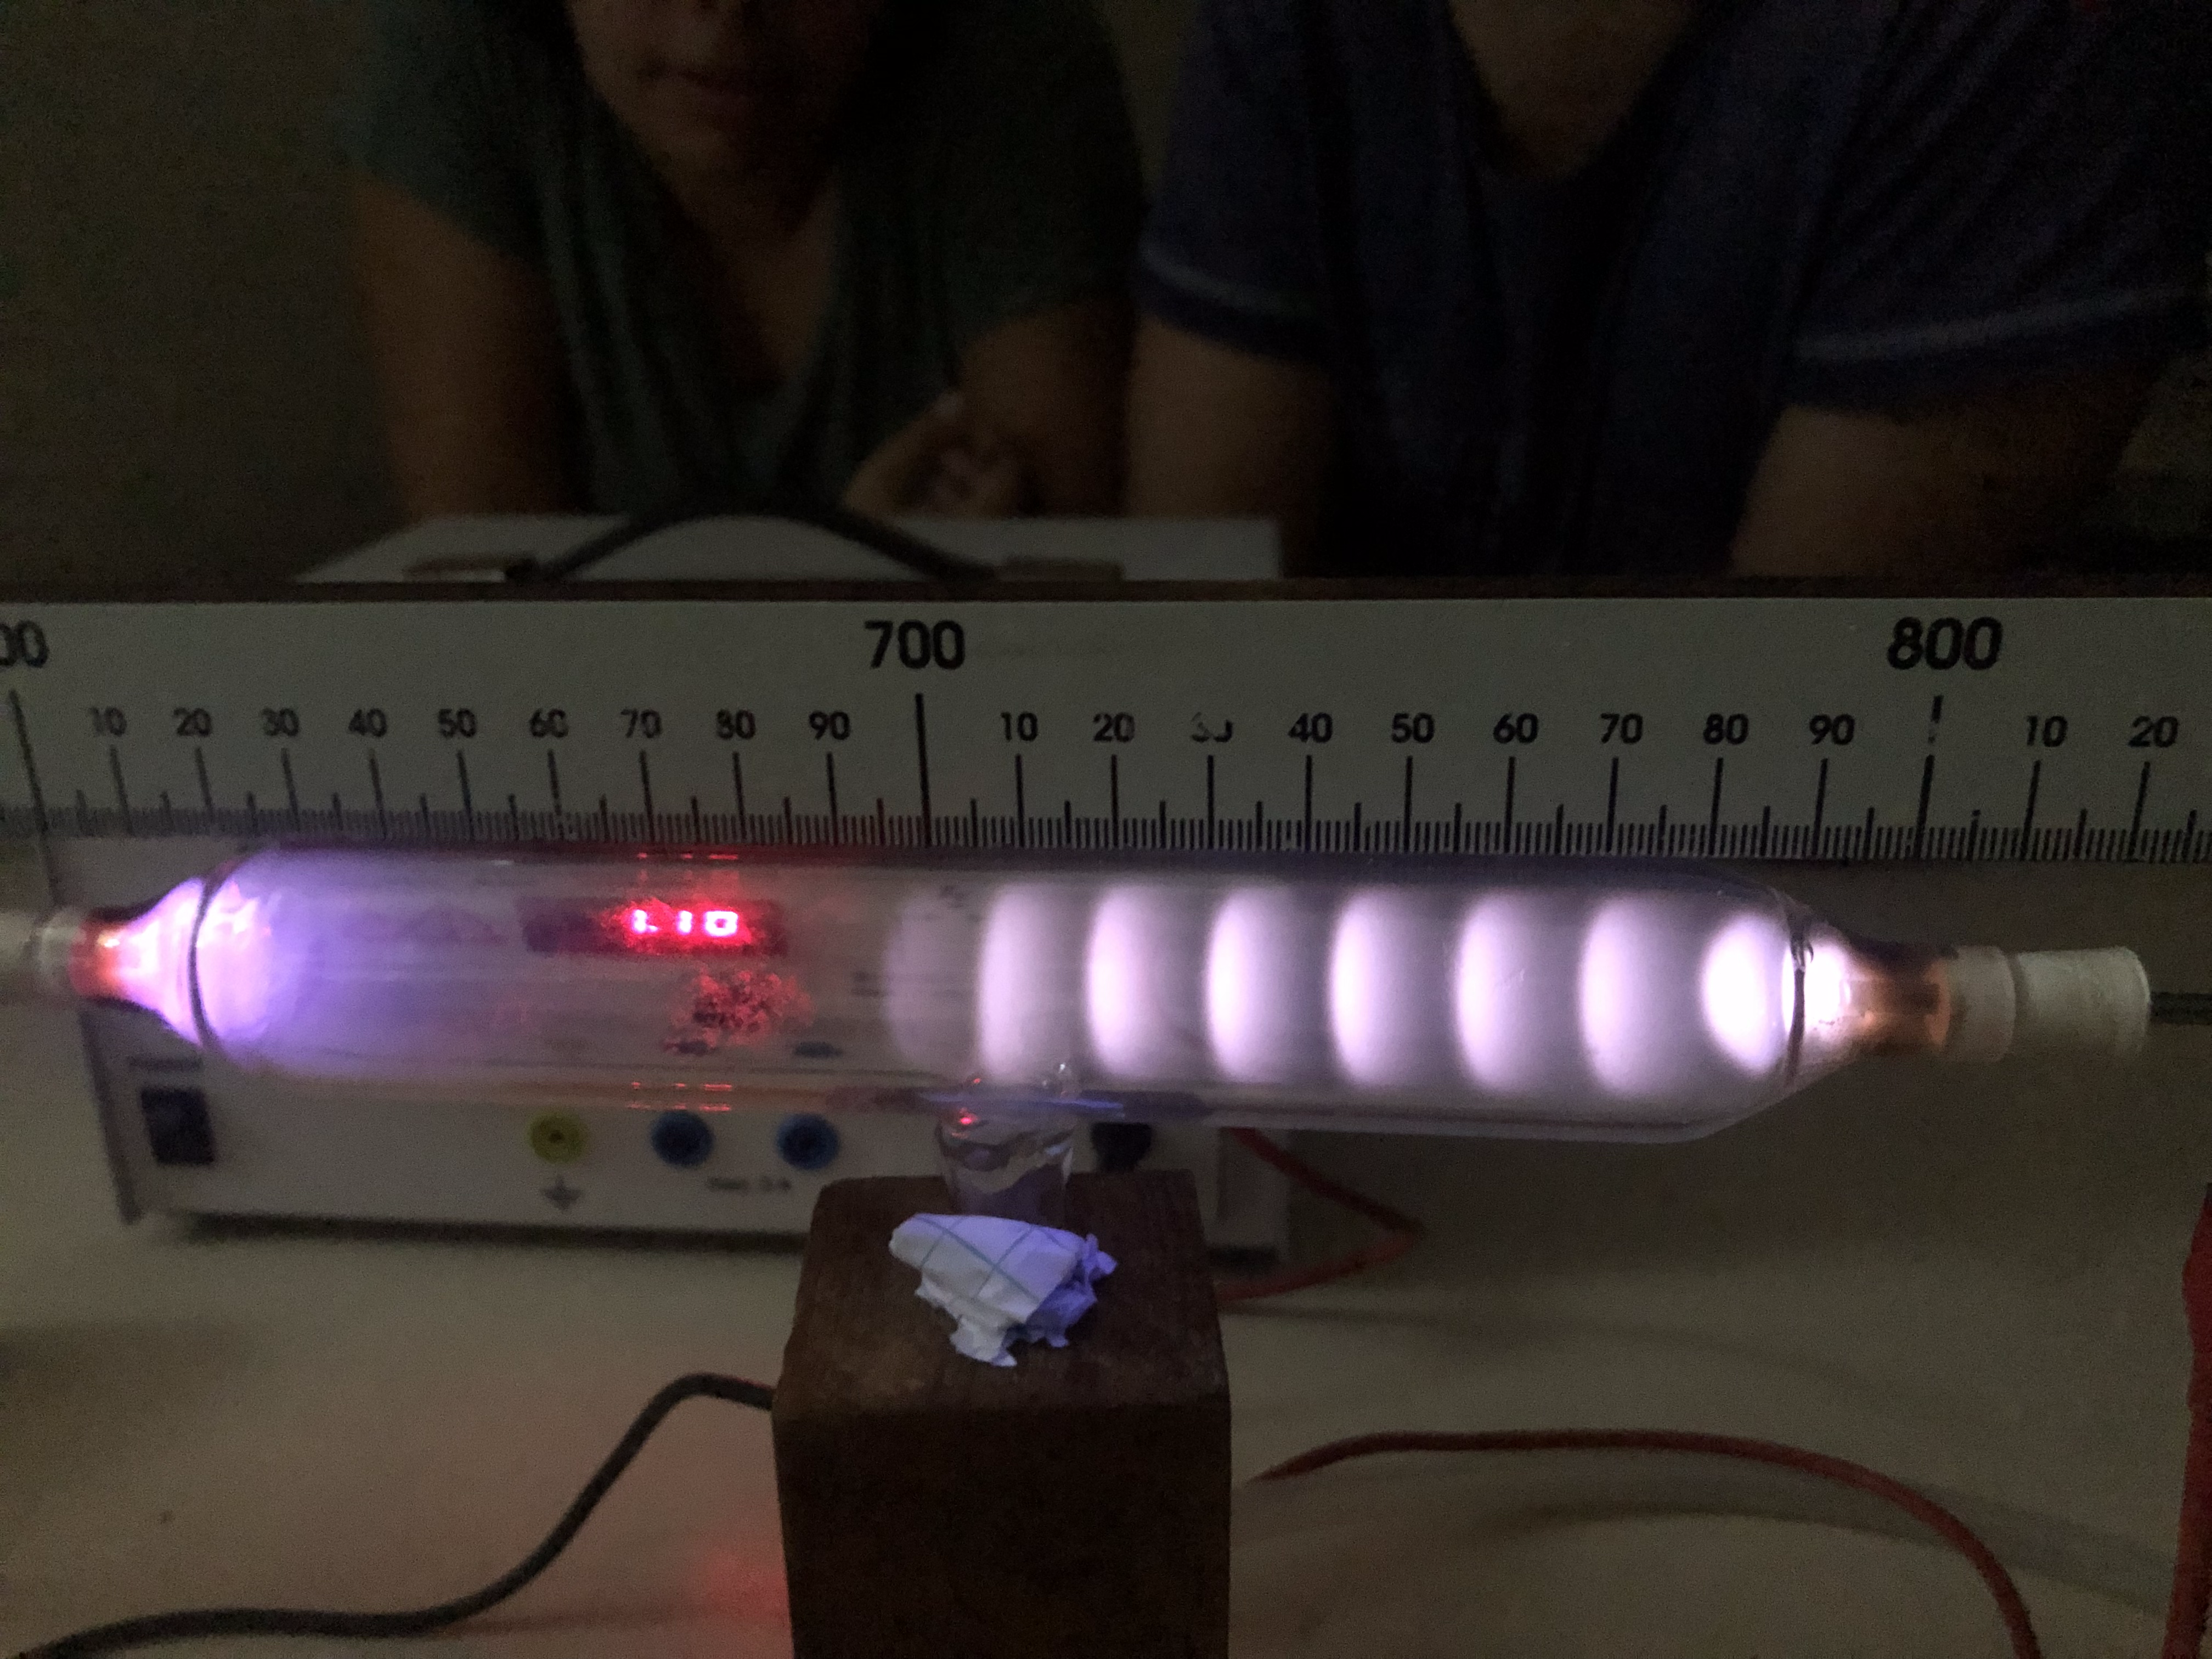
\includegraphics[width=0.5\linewidth]{Fig1.png}
    \caption{Modelo de pequenos sinais $ac$.}
    \label{fig:Fig1}
\end{figure}

\begin{figure}[h]
    \centering
    \includegraphics[width=0.5\linewidth]{Fig2.png}
    \caption{Circuito para grandes sinais equivalentes validos quando o transistor está na região de ativação direta.}
    \label{fig:Fig2}
\end{figure}

O ganho do emissor comum com carga resistiva é dado por:
\begin{equation}
    A_{\nu}=-g_{m}\cdot(R_{C}//r_{0})\implies|A_{\nu}|=\frac{I_{C}\cdot(R_{C}//r_{0})}{V_{T}}
\end{equation}

Se o circuito for polarizado de tal forma a proporcionar a maior excursão possível do sinal de saída ($V_{CEO}\approx\frac{V_{CC}}{2}$), e pudermos desprezar $r_{0}$ comparado com $R_{C}$, o ganho deste circuito fica sendo dado por:
\begin{equation}
    |A_{\nu}|=\frac{I_{C}\cdot R_{C}}{V_{T}}=\frac{1}{2}\frac{V_{CC}}{V_{T}}
\end{equation}

Para $V_{T}=26$ mV, então obtemos,
\begin{equation}
    |A_{\nu}|\approx20\cdot V_{CC}
\end{equation}

Portanto, ao se polarizar o circuito para obter excursão máxima de sinal, o ganho fica limitado pela fonte de alimentação, não importando os valores de $R_{C}$ e $I_{C}$.

As impedâncias de entrada e saída deste circuito são facilmente calculadas por inspeção no modelo de pequenos sinais. A corrente na entrada do transistor $I_{i}$ é dada por:
\begin{equation}
    I_{i}=\frac{V_{i}}{r_{\pi}}
\end{equation}

A impedância vista na base de $Q_{1}$ é simplesmente:
\begin{equation}
    Z_{i}=\frac{V_{i}}{I_{i}}=r_{\pi}=\beta\cdot\frac{V_{T}}{I_{C}}
\end{equation}

A impedância de saída (calculada com a entrada em curto). é:
\begin{equation}
    Z_{0}=r_{0}//R_{C}
\end{equation}

Já que com a entrada em curto, a fonte de corrente controlada $g_{m}\cdot \nu_{I}$ é igual a zero. O ganho de corrente (com a saída em curto), $A_{i}=\frac{I_{0}}{I_{i}}$, é o próprio ganho $\beta_{ac}$ do transistor.

É bastante instrutivo fazer uma simulação de um amplificador emissor comum e comparar os parâmetros obtidos através do SPICE e os calculados através do modelo.

\begin{figure}[h]
    \centering
    \includegraphics[width=0.5\linewidth]{Fig3.png}
    \caption{Modelo de um amplificador emissor comum.}
    \label{fig:Fig3}
\end{figure}

\begin{figure}[h]
    \centering
    \includegraphics[width=0.5\linewidth]{Fig4.png}
    \caption{Modelo SPICE para comparação com amplificador emissor comum.}
    \label{fig:Fig4}
\end{figure}




%%%%%%%%%%%%%%%%%%%%%%%%%%%%%%%%%%%%%%%%%%%%%%%%%%%%%%
\section{Procedimento experimental}\label{Sec 3 - Experimento}
O experimento como um todo foi realizado em três etapas. Na primeira montou-se um circuito amplificador emissor comum como ilustrado na Figura (\ref{fig:Fig3}). Já na segunda se investigou o comportamento do mesmo como um amplificador emissor comum. Por fim, na terceira etapa foi realizada uma simulação usando o programa \href{https://docente.ifrn.edu.br/leonardoteixeira/links/instalador-do-circuitmaker-student/view}{\texttt{CircuitMaker}} utilizando os mesmos componentes e instrumentos utilizados na experiência no laboratório. A comparação entre os dados experimentais e a simulação se encontra na seção \ref{Sec 4 - Resultados}. 

Abaixo está listado os materiais utilizados nas duas etapas do experimento:
\begin{enumerate}
    \item 1 gerador de funções AGF1022 da Tektronix;
    \item 1 osciloscópio digital TDS11002B da Tektronix;
    \item 1 protoboard de duas seções;
    \item 2 capacitores de $1\mu$F;
    \item 1 resistor de 300 $\Omega$;
    \item 1 resistor de 10k $\Omega$;
    \item 1 resistor de 6.7 $\Omega$;
    \item 1 resistor de 560 $\Omega$;
    \item 1 transistor BC547;
    \item um porta pilhas de duas seções.
\end{enumerate}

Vamos agora descrever o procedimento experimental em cada etapa.

\subsection{Etapa 1: Amplificador Emissor Comum}\label{Etapa 1}
\begin{enumerate}
    \item Primeiramente montou-se um circuito do tipo amplificador emissor comum como ilustrado na Figura (\ref{fig:Fig3}).
    \begin{itemize}
        \item Circuito montado segundo o esquema exposto na Figura (\ref{fig:Fig3}):
        \begin{figure}[h!]
            \centering
            \includegraphics[width=0.5\linewidth]{Circuito.jpeg}
            \caption{Circuito montado seguindo o esquema de um amplificador do tipo emissor comum.}
            \label{fig: Sinais 1 e 2}
        \end{figure}
    \end{itemize}
    
    \item Em seguida, capturou-se o sinal amplificado no canal 1, e o sinal de entrada no canal 2 no osciloscópio. O osciloscópio foi colocado para operar no modo Xt.
    \begin{itemize}
        \item Sinais capturados nos canais 1 e 2 do osciloscópio:
        \begin{figure}[h!]
            \centering
            \includegraphics[width=0.5\linewidth]{Sinais.jpeg}
            \caption{Sinal de entrada do osciloscópio (azul) e sinal amplificado (amarelo).}
            \label{fig: Sinais 1 e 2}
        \end{figure}
    \end{itemize}
\end{enumerate}

\subsection{Etapa 2: Simulação da Etapa 1 usando o \texttt{CircuitMaker}}
\begin{enumerate}
    \item Semelhantemente ao que foi feito na etapa anterior, foi criado um arquivo na extensão \texttt{.CKT} intitulado \texttt{Amplificators.ckt} onde foi montado um circuito como descrito na etapa 1, subseção \ref{Etapa 1}.
    \begin{figure}[h!]
        \centering
        \includegraphics[width=0.5\linewidth]{Fig5.png}
        \caption{Circuito do amplificador emissor comum.}
        \label{fig: Circuit_Maker}
    \end{figure}
    
    \item E da mesma forma como foi feito na etapa anterior, avaliou-se o sinal de saída do amplificador:
    %\begin{figure}[h]
    %    \centering
    %    \includegraphics[width=0.5\linewidth]{}
    %    \label{fig:Circuit_Maker-Result}
    %\end{figure}
\end{enumerate}



%%%%%%%%%%%%%%%%%%%%%%%%%%%%%%%%%%%%%%%%%%%%%%%%%%%%%%
\section{Análise dos resultados}\label{Sec 4 - Resultados}
Nesta seção iremos discutir os resultados obtidos ao longo das etapas experimentais descritas anteriormente.

Como descrito na seção \ref{Sec 2 - Teoria}, a ideia dos transistores é a de amplificação de um sinal do tipo AC, respectivamente. Dessa forma, note que o sinal amarelo condiz é justamente o sinal de entrada (azul) amplificado.


Com relação ao modelo teórico obtido por meio de uma simulação através do programa \texttt{CircuitMaker}, temos algumas semelhanças. Primeiramente, note que como o \texttt{CircuitMaker} é um programa que simula a parte teórica dos componentes eletrônicos, ele irá simular apenas o funcionamento dos amplificadores tendo como sinal de entrada uma onda senoidal com uma frequência específica constante e não um conjunto de frequências variadas. Dessa forma, vemos que o modelo teórico exprime muito bem o caráter esperado para os amplificadores.



%%%%%%%%%%%%%%%%%%%%%%%%%%%%%%%%%%%%%%%%%%%%%%%%%%%%%%
\section{Conclusões}\label{Sec 5 - Conclusão}
Dado o exposto ao longo deste relatório, temos que os resultados experimentais expostos na seção \ref{Sec 3 - Experimento} condizem com o modelo matemático exposto na seção \ref{Sec 2 - Teoria}. Portanto, temos que os resultados experimentais estão dentro do esperado do modelo teórico a menos de alguns ruídos experimentais, mostrando assim que os modelos teóricos para amplificadores do tipo emissor comum exprimem razoavelmente os amplificadores emissores comuns reais.



%%%%%%%%%%%%%%%%%%%%%%%%%%%%%%%%%%%%%%%%%%%%%%%%%%%%%%
\begin{thebibliography}{100}

\bibitem{Spitzer}
Spitzer, Frank; Howarth (1973). \textit{Principles of Modern Instrumentation}. Nova York: [s.n.] p. Ch. 11

\bibitem{Sedra}
SEDRA, Adel S., \textit{Microeletrônica} 5º ed. volume único, Prentice Hall, 1997

\bibitem{Bakshi}
Bakshi, U.A.; Bakshi, A.V., \textit{Circuit Analysis - II}, Technical Publications, 2009 \texttt{ISBN 9788184315974}.

\bibitem{Horowitz}
Horowitz, Paul; Hill, Winfield, \textit{The Art of Electronics} (3rd edition), Cambridge University Press, 2015 \texttt{ISBN 0521809266}.

\end{thebibliography}

\end{document}